% GENERATED from archived economic results by build_economic_figures.py.
% Actual customers and receipts remain zero; all monetary results below are simulated.

\subsection{Frozen results: the unit contributes, the enterprise loses}

The initial confirmation contains 3,584 worlds; the revised confirmation contains
7,168 worlds, with 256 worlds per policy--scenario cell. The original best active
training policy was the \USD{349} subscription. After the revision, the precommitted
rule still selects \textbf{stop}. The commitment gate is the least-loss spending
policy, but no spending policy qualifies as profitable.

In the fresh base worlds, the \USD{449} instrument produces mean revenue of
\USD{5,399.72} and mean total contribution of \USD{4,145.41}. Contribution
per net retained order averages \USD{339.84} across world-level ratios; this is a conditional modeled
commercial margin, not a measured market price. The enterprise delivers only
12.14 retained orders over 7.01 active months on average. Its recurring
operating result is \(-\)\USD{17,997.71}; including the launch expense, its
full-project result is \(-\)\USD{26,397.71}. Figure~\ref{fig:economic-bridge}
shows why a large per-order margin is insufficient.

\begin{figure}[htbp]
\centering
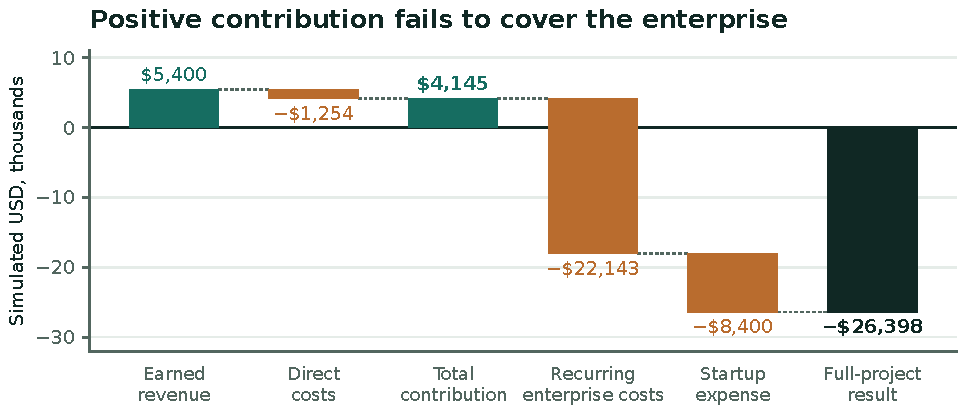
\includegraphics[width=\linewidth]{figures/economic_cost_bridge.pdf}
\caption{Mean simulated base-case cost bridge for the qualified \USD{449}
instrument, 256 worlds. Revenue is net of refunds. Direct costs include failed
attempts, retries, processing, support and bad debt. Recurring costs include acquisition and
\USD{1,200} equipment depreciation; the separate \USD{8,400} startup expense
therefore avoids counting equipment twice. Initial startup cash outlay is
\USD{9,600}. Figure labels are rounded; the prose and ledger retain exact cents.}
\label{fig:economic-bridge}
\end{figure}

The subscription has a higher mean number of retained orders (19.37), but
still loses \USD{26,521.09} over the full project. The instrument's simulated
acquisition cost, including allocated sales labor, averages \USD{557.68} per buyer,
against \USD{410.88} lifetime contribution within the observed \emph{simulated}
history. Neither model produces enough accepted demand to absorb the complete
enterprise cost. Every operating confirmation history loses money; none repays startup or
continues for the entire 24-month operating window.

\subsection{Stress outcomes and the meaning of survival}

\begin{table}[htbp]
\centering\small
\begin{tabularx}{\linewidth}{@{}Yrrr@{}}
\toprule
Scenario & \shortstack{Qualified\\\USD{449}} & \shortstack{Subscription\\\USD{349}} & \shortstack{Commitment gate\\\USD{449}} \\
\midrule
Base & $-26{,}397.71$ & $-26{,}521.09$ & $-3{,}050.00$ \\
Competitive pressure & $-26{,}468.83$ & $-26{,}484.97$ & $-3{,}050.00$ \\
Demand shortfall & $-26{,}431.52$ & $-26{,}569.31$ & $-3{,}050.00$ \\
Supplier disruption & $-26{,}449.16$ & $-26{,}508.49$ & $-3{,}050.00$ \\
Cost inflation & $-25{,}218.99$ & $-25{,}405.01$ & $-3{,}725.00$ \\
Late payments & $-25{,}264.48$ & $-26{,}521.09$ & $-3{,}050.00$ \\
Combined downside & $-27{,}280.16$ & $-26{,}825.40$ & $-3{,}522.50$ \\
\bottomrule
\end{tabularx}
\caption{Mean simulated full-project profit in USD after all stated costs and
the assumed tax treatment. Each cell contains 256 fresh worlds. The stop policy,
omitted from the table, preserves initial capital and earns zero. No table entry
is realized revenue, a buyer quote, or evidence of willingness to pay.}
\label{tab:economic-stress}
\end{table}

All spending policies lose in every reported world, including the gate's search
expense when it does not launch. Insolvency frequency is zero: the operating
policies shut down before exhausting their reserve, and the revised gate does not
launch. This is loss containment, not sustainable cash generation. Cost inflation
can cause a smaller total loss by forcing earlier closure and fewer deliveries;
it does not improve the business. Late payment leaves the prepaid subscription
unchanged, making clear that invoice timing is not its binding commercial defect.

The base instrument's tenth percentile of profit is \(-\)\USD{27,456.34};
its ninetieth percentile is \(-\)\USD{25,449.74}. These percentiles describe
variation inside the authored economy. They cannot quantify uncertainty about
whether the assumed customer population or preferences exist.

\subsection{The revision improves the decision without inventing customers}

At the frozen base costs, the launch condition requires 57 simultaneous qualifying
commitments. The revised search obtains a mean peak of 4.32 and a maximum of 11
across the 256 base worlds. It launches in \textbf{0/256} worlds, earns no revenue,
and spends \USD{2,850} on search plus \USD{200} on closeout. Its unconditional
project loss is therefore \USD{3,050}; profit conditional on launch is
\texttt{null}, because the conditioning event never occurs.

\begin{figure}[H]
\centering
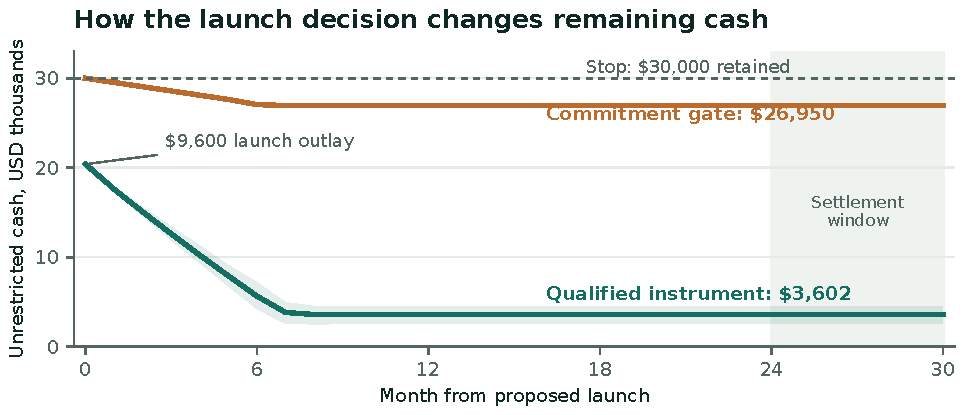
\includegraphics[width=\linewidth]{figures/economic_cash_paths.pdf}
\caption{Base-case unrestricted cash: means with pointwise tenth--ninetieth
percentile bands across the 256 synthetic worlds. The narrow gate path reflects
the same bounded search expenditure in every base world. The qualified offer
closes after a mean 7.01 active months; its terminal mean cash is
\USD{3,602.29}. The final six months settle outstanding obligations. No refundable
customer custody is spent on operations.}
\label{fig:economic-cash}
\end{figure}

The intervention succeeds at preserving more of the \USD{30,000} initial equity.
It does not establish a profitable commercial opening. The frozen rule's stop
decision is economically preferable to paying for a presale search that the
current assumptions predict will fail; neither decision satisfies Proof~II.

\subsection{Sensitivity and the limits of the economic evidence}

The static qualified-product calculation allocates construction, recurring costs,
requalification and closeout into about \USD{3,431.67} per month. At a nominal
\USD{449}, its expected contribution is \USD{345.81} per retained order, versus
the dynamic histories' mean of \USD{339.84}; the fixed-volume calculation omits
strategic price erosion and negotiated discounts. Approximately ten retained
orders per month would cover its burden, yielding only about \USD{634} pretax
over 24 months under constant-volume arithmetic. At \USD{349} the threshold
rises to fourteen orders, and at \USD{249}
to twenty-three. These are conditional thresholds, not jointly demonstrated
price--volume possibilities. Dynamic competition, acquisition, refunds and scope
refusal prevent the executed economy from reaching them.

A separate 40/80/160-hour replacement-construction sensitivity uses 32 new worlds
per policy and cost level. Both original operating policies continue to lose and
the commitment gate still refuses launch. Its control of timing helps preserve
capital without improving the unobserved willingness-to-pay premise. A large,
fully aware synthetic cohort was used only to exercise the simulator's launch
and positive-profit code branches; it is not an economic success scenario.

The corrected Decimal audit performs \textbf{3,512,320} monetary checks on the
revised confirmation and passes again under optimized Python. Twenty-one
archived participant traces replay exactly, and unchanged native AGI ALPHA code
agrees on 21 aggregate cash bridges. An original counter incorrectly included a
prior-month check in month zero; the original records and an explicit correction
are retained. Only that audit counter changed after confirmation, verified by an
AST comparison; no policy, outcome or money path changed. These checks establish
reproducible accounting within the model, not empirical demand or actual profit.

